\documentclass[letterpaper, 10 pt, conference]{ieeeconf} 
\IEEEoverridecommandlockouts
% The preceding line is only needed to identify funding in the first footnote. If that is unneeded, please comment it out.
\usepackage{multirow}%,bigdelim}
\usepackage[hidelinks,draft]{hyperref} % draft is added to bypass issues seen with glossary terms broken up by line-breaks
\newcommand{\emaillink}[1]{\href{mailto:#1}{#1}}
\usepackage{url}
\usepackage{soul}
\usepackage{cite}
\usepackage{amsmath,amssymb,amsfonts}
\usepackage{mathtools}
\usepackage{siunitx}
\usepackage{xfrac}
% \usepackage{algorithmic}
\usepackage{graphicx}
\graphicspath{{figs/}}
\usepackage{tcolorbox}
\usepackage{textcomp}
\usepackage{xcolor}
\usepackage{siunitx}
\usepackage{xspace}
\usepackage[utf8]{inputenc}

% \usepackage{tablefootnote}
\usepackage[export]{adjustbox}

% tables
\usepackage{booktabs}
\usepackage{multirow}
\usepackage{makecell}

% Spacing
\usepackage[final]{microtype} % font expansion + protrusion

% \setlist[description]{leftmargin=\parindent,labelindent=\parindent}
\def\BibTeX{{\rm B\kern-.05em{\sc i\kern-.025em b}\kern-.08em
    T\kern-.1667em\lower.7ex\hbox{E}\kern-.125emX}}
\usepackage[textsize=tiny]{todonotes}
% \usepackage[textsize=tiny,disable]{todonotes}
% Maximize margin width to still barely see the sides of todonotes
\setlength{\marginparwidth}{1.5cm}

% Define a todolist for checkboxes
\makeatletter
\let\labelindent\relax
\makeatother
\usepackage[inline]{enumitem}
\newlist{todolist}{itemize}{2}
\setlist[todolist]{label=$\square$}
\usepackage{pifont}
\newcommand{\cmark}{\ding{51}}%
\newcommand{\xmark}{\ding{55}}%
\newcommand{\done}{\rlap{$\square$}{\raisebox{2pt}{\large\hspace{1pt}\cmark}}%
\hspace{-2.5pt}}
\newcommand{\wontfix}{\rlap{$\square$}{\large\hspace{1pt}\xmark}}

% \ifCLASSOPTIONcompsoc
%   \usepackage[caption=false,font=normalsize,labelfont=sf,textfont=sf]{subfig}
% \else
%   \usepackage[caption=false,font=footnotesize]{subfig}
% \fi
\usepackage[caption=false,font=footnotesize]{subfig}
\usepackage{titlecaps}
\usepackage{algorithm,algpseudocode}

%%%%%%%%%%%%%%%%%%%%%%%%%%%%%%%%%%%%%%%%%%%%%%%%%%
% Common macros
%%%%%%%%%%%%%%%%%%%%%%%%%%%%%%%%%%%%%%%%%%%%%%%%%%

\newcommand{\hsia}{H-Si(100)-2$\times$1\@\xspace}
\newcommand{\hsib}{H-Si(111)-1$\times$1\@\xspace}

% referencing labels
\newcommand{\fref}[1]{Fig.~\ref{#1}}
\newcommand{\frefplain}[1]{Fig.~#1}
\newcommand{\tref}[1]{Table~\ref{#1}}
\newcommand{\secref}[1]{Section~\ref{#1}}
\newcommand{\eref}[1]{Eq.~\eqref{#1}} %\eqref provided by amsmath
\newcommand{\appenref}[1]{Appendix~\ref{#1}}

% in-text functions
\newcommand{\tsps}[1]{\textsuperscript{#1}}  % text superscripts
\newcommand{\tsbs}[1]{\textsubscript{#1}}  % text superscripts
\newcommand{\sref}[1]{\protect\subref{#1}}  % subfig referencing in main caption
\newcommand{\bpar}[1]{(\textbf{#1})}        % bolt text in parentheses

% To-do items
\newcommand{\TODO}[1]{\textcolor{red}{TODO: #1}}
\newcommand{\TODOlow}[1]{\textcolor{blue}{TODO: #1}}
\newcommand{\PLAN}[1]{
    \begin{tcolorbox}[colback=blue!30!white, % Background color
                      colframe=blue!60!black, % Frame color
                      boxsep=1pt, % Box padding
                      arc=2pt, % Corner rounding
                      boxrule=1pt] % Frame thickness
        \tiny
        #1
    \end{tcolorbox}
}
\newcommand{\OLD}[1]{\textcolor{lightgray}{#1}}

% math operators
\DeclareMathOperator\erf{erf}
\DeclarePairedDelimiter\ceil{\lceil}{\rceil}
\DeclarePairedDelimiter\floor{\lfloor}{\rfloor}
\newcommand{\vect}[1]{\boldsymbol{\mathbf{#1}}}
\DeclareSIUnit\angstrom{\text {Å}}

% Terms/math
\newcommand{\etal}{\textit{et al.}}

% \renewcommand{\baselinestretch}{0.99}

% Make \gls output with first letter of each word capitalized, not just first word
\usepackage{mfirstuc}

\makeatletter
\let\oldmakefirstuc\makefirstuc
\renewcommand*{\makefirstuc}[1]{%
  \def\gls@add@space{}%
  \mfu@capitalisewords#1 \@nil\mfu@endcap
}
\def\mfu@capitalisewords#1 #2\mfu@endcap{%
  \def\mfu@cap@first{#1}%
  \def\mfu@cap@second{#2}%
  \gls@add@space
  \oldmakefirstuc{#1}%
  \def\gls@add@space{ }%
  \ifx\mfu@cap@second\@nnil
    \let\next@mfu@cap\mfu@noop
  \else
    \let\next@mfu@cap\mfu@capitalisewords
  \fi
  \next@mfu@cap#2\mfu@endcap
}
\makeatother

\usepackage[acronym]{glossaries}

% Disable hyperlinks for glossary entries
\glsdisablehyper

% ML
\newacronym{ai}{AI}{Artificial Intelligence}
\newacronym{ml}{ML}{Machine Learning}
\newacronym{llm}{LLM}{Large Language Model}
\newacronym{qat}{QAT}{Quantization-Aware Training}
\newacronym{api}{API}{Application Programming Interface}

% ML Accel
\newacronym{mvm}{MVM}{Matrix-Vector Multiplication}
\newacronym{mxu}{MXU}{Matrix Multiply Unit}
\newacronym{mac}{MAC}{Multiply-Accumulate}

% Atomic/Nanotech/Physics
\newacronym{stm}{STM}{Scanning Tunneling Microscope}
\newacronym{afm}{AFM}{Atomic Force Microscope}
\newacronym{set}{SET}{Single-Electron Transistor}
\newacronym{bdl}{BDL}{Binary-Dot Logic}

% Field-Coupled Nanocomputing
\newacronym{fcn}{FCN}{Field-Coupled Nanocomputing}
\newacronym{sidb}{SiDB}{Silicon Dangling Bond}
\newacronym{qca}{QCA}{Quantum-dot Cellular Automata}
\newacronym{nml}{NML}{NanoMagnetic Logic}

% Devices
\newacronym{hal}{HAL}{Hardware Abstraction Layer}
\newacronym{pi}{PI}{Primary-Input}
\newacronym{io}{I/O}{Input/Output}
\newacronym{adc}{ADC}{Analog-to-Digital Converter}
\newacronym{cmos}{CMOS}{Complementary Metal-Oxide-Semiconductor}
\newacronym{cad}{CAD}{Computer-Aided Design}
\newacronym{tpu}{TPU}{Tensor Processing Unit}
\newacronym{alu}{ALU}{Arithmetic Logic Unit}

% Architecture
\newacronym{pe}{PE}{Processing Element}

% EDA
\newacronym{rtl}{RTL}{Register-Transfer Level}
\newacronym{eda}{EDA}{Electronic Design Automation}
\newacronym{aig}{AIG}{And-Inverter Graph}

% fiction-specific algorithms
\newacronym{gold}{\emph{gold}}{Graph-Oriented Layout Design}
\newacronym{plo}{\emph{PLO}}{Post-Layout Optimization}

% Others
\newacronym[longplural={Figures of Merit}]{fom}{FoM}{Figure of Merit}


% solve error: Page 1 has margin impositions
\def\IEEEtitletopspace{18pt}

\clubpenalty = 10000
\widowpenalty = 10000
\displaywidowpenalty = 10000

\begin{document}

\title{RTL-to-Atoms Synthesis of an Atomic-Scale Machine Learning Accelerator with Technology-Specific Optimizations}

% \author{%
%     Samuel~S.~H.~Ng, %
%     Marcel Walter, %
%     Jan Drewniok, %
%     Simon Hofmann, %
%     Robert Wille, %
%     and Konrad Walus%
%     \thanks{This work was supported by the Natural Sciences and Engineering Research Council of Canada under Grant \mbox{RGPIN-2022-04830}.}%
%     \thanks{S.~S.~H.~Ng and K.~Walus were with the Department of Electrical and Computer Engineering, University of British Columbia, Vancouver, BC, Canada (\mbox{\{samueln, konradw\}@ece.ubc.ca}); M.~Walter, J.~Drewniok, S.~Hofmann, and R.~Wille were with the Chair for Design Automation, Technical University of Munich, BY, Germany (\mbox{\{marcel.walter, jan.drewniok, simon.t.hofmann, robert.wille\}@tum.de}). M.~Walter, S.~Hofmann, and R.~Wille were also with the Munich Quantum Software Company GmbH, Garching near Munich, BY, Germany. R.~Wille was also with the Software Competence Center Hagenberg (SCCH) GmbH, Hagenberg, O\"O, Austria.}%
% }

% \author{Anonymous author(s)}

\maketitle

\begin{abstract}
%
\TODO{}
% At a time when traditional CMOS technologies approach their fundamental scaling limits and artificial intelligence continues to escalate global computational demands, emerging post-CMOS technologies like \glspl{sidb} provide promising pathways towards energy-efficient computation.
% \glspl{sidb} offer atomic-scale precision and discrete charge control, enabling the realization of ultra-dense computational logic. However, manual layout design and verification have historically restricted the exploration and scalability of \gls{sidb}-based logic systems.
% To this end, this work demonstrates an automated, end-to-end \gls{eda} flow for designing and synthesizing a core component of a \gls{mxu} from high-level \gls{rtl} Verilog descriptions down to dot-accurate \gls{sidb} layouts. Leveraging recent advances in \gls{sidb}-focused \gls{eda} tooling, we demonstrate the first fully automated design flow capable of translating \gls{rtl} descriptions into manufacturable quantum-dot layouts. The proposed hierarchical Verilog approach addresses existing \gls{eda} constraints while facilitating comprehensive operational verification via test benches. Additionally, our design process incorporates reliability-focused \glspl{fom}, ensuring the selection of robust logic gates throughout synthesis.
% Our synthesized \gls{mxu} \gls{pe} layout represents a significant milestone in \gls{sidb} logic design, bridging previously manually-intensive workflows with scalable, automated methodologies. Despite achieving larger footprints than hand-crafted designs, the presented approach provides a valuable foundation for future optimization and widespread adoption of \gls{sidb}-based computing architectures.
%
\end{abstract}

% \begin{IEEEkeywords}
% Computer aided design, machine learning acceleration, quantum dots, silicon dangling bonds, simulation
% \end{IEEEkeywords}


\glsresetall

\section*{Extension Plan}

\subsection*{Main objectives}

Objectives that, together, satisfy \SI{50}{\percent} new contents rule:
%
\begin{todolist}
    \item[\done] Implement ripple-carry adder and array multiplier in Verilog with a wrapper that automatically generates N-bit versions
    \item[\done] Testbench the above for verification
    \item[\done] In the Processing Element, replace multiplication and accumulation operations with the optimized \glspl{alu}
    \item[\done] Synthesize and report changes
    \item New table similar to DATE's table: report multiple algorithm combinations (e.g., ortho with and without PLO, FoM vs. uniform gates), also report FoM-informed results similarly
    \item Create multi-attempt averaged score benchmark set:
    \begin{itemize}
        \item To clarify, this is an attempt at realizing that ``scientifically rigorous'' synthesis results comparison
        \item We can create a long-running script that makes $N$ attempts at deepsyn, TM to FoM-informed and uniform gates, $M$ attempts at \emph{gold} (if tractable). Since \emph{PLO} is deterministic we won't have to rerun that. This means $2 \cdot N \cdot M$ attempts in total. Missing anything?
    \end{itemize}
\end{todolist}

\subsection*{Stretch goals}

Only do if there's time and if it's worth it:
%
\begin{todolist}
    \item Add half-adder gate to technology mapper
    \begin{itemize}
        \item IMO probably worth it but pending TUM's confirmation
    \end{itemize}
    \item If there's time, also try to improve the pin-routing area estimation (either by hand or by auto routing if available)
    \begin{itemize}
        \item IMO more time consuming and possibly not worth it
    \end{itemize}
\end{todolist}

%%%%%%%%%%%%%%%%%%%%%%%%%%%%%%%%%%%%%%%%%%%%%%%%%%
% Introduction
%%%%%%%%%%%%%%%%%%%%%%%%%%%%%%%%%%%%%%%%%%%%%%%%%%
\section{Introduction} \label{sec:intro}

\OLD{As CMOS scaling faces increasing barriers and challenges, and with global energy demands rapidly escalating due to the widespread adoption of artificial intelligence across diverse application domains, there is renewed urgency to develop highly energy-efficient computing hardware. \gls{fcn} has emerged as a compelling alternative for post-CMOS logic systems, where logic states encoded in the position of charges in quantum dots~\cite{lent2003molecular,ardesi2024modeling} or the magnetic polarity of nano-magnets~\cite{bernstein2005magnetic,giri2016modeling} enable computation and signal transmission through local field interactions. Among the various \gls{fcn} implementation options, \glspl{sidb} stand out as a promising candidate due to their ability to be fabricated at atomically precise locations~\cite{huff2017atomic, achal2018lithography, pitters2024atomically} and their discretely controllable charge states~\cite{haider2009controlled, pitters2011charge}.
Following a successful experimental demonstration of an \gls{sidb} OR gate measuring $5 \times \SI{6}{\nm^2}$~\cite{huff2018binary}, \gls{cad} tools supporting different levels of \gls{sidb} logic exploration have emerged. On the physical design level, the introduction of \emph{SiQAD}~\cite{ng2020siqad} and an ecosystem of specialized simulators~\cite{chiu2020poissolver, drewniok2023quicksim, drewniok2024need} allow users to create and simulate \gls{sidb} systems.}

\OLD{The advent of \gls{sidb} \gls{cad} capabilities has spurred research interest into designing \gls{sidb} logic gates and circuits~\cite{vieira2022threeinput, bahar2020design, ahmadpour2023energyaware}, where designers carefully designed quantum-dot layouts in SiQAD and verify their behavior with SiQAD's physical simulation capabilities~\cite{ng2020siqad, chiu2020poissolver, drewniok2023quicksim, drewniok2024need}. However, the fully manual design flow of these layouts caused them to be time-consuming ordeals. Fortunately, innovations that introduce automation to multiple levels of the \gls{sidb} design flow opened new pathways for large-scale \gls{sidb} logic implementation and studies. At the quantum-dot level, automated \gls{sidb} gate designers~\cite{lupoiu2022automated, drewniok2023minimal} have enabled the creation of standard-tile libraries~\cite{walter2022hexagons, ng2024unlocking}. The implementation of \gls{sidb} support to \emph{fiction}~\cite{walter2019fiction}, a state-of-the-art \gls{eda} framework specialized for \gls{fcn} systems, has enabled higher-level exploration of \gls{sidb} applications by automating the synthesis from gate-level netlists---structured descriptions of digital circuits composed of interconnected logic gates---down to dot-accurate \gls{sidb} layouts at scales impractical for manual design.}

\OLD{Prior to the availability of \gls{sidb} \gls{eda} tools, the time-consuming nature and difficulty of scaling up \gls{sidb} designs had also limited existing research into large-scale \gls{sidb} applications.
Among published \gls{sidb} applications is a \gls{mxu} which is inspired by Google's \gls{tpu}~\cite{ng2023blueprint, jouppi2017indatacenter}, where the designer used simulation-proven \gls{sidb} logic components (up to a half-adder) to extrapolate and approximate the area cost and performance figures of a full \gls{sidb} \gls{mxu}.
To move beyond approximations and toward practical implementation, we realize the \gls{mxu} in \gls{rtl} Verilog---a high-level hardware description language commonly used to define digital circuits through clear, structured specifications of data flow and control logic between hardware registers. Leveraging state-of-the-art \gls{eda} tools, our \gls{rtl} implementation can be automatically synthesized into dot-accurate \gls{sidb} layouts, enabling a fully automated, scalable, and verifiable end-to-end \gls{sidb} design flow---from \gls{rtl} descriptions, through logic synthesis and optimization, down to quantum-dot layouts.
To our knowledge, this represents the first realization of a practically relevant \gls{sidb} application design flow validated at every step from \gls{rtl} description to manufacturable layout, thus setting a crucial benchmark for future \gls{sidb} application development and validation.}
\TODO{This article substantially extends our IEEE NANO 2025 paper \cite{ng2025building} by: (i) … (new idea), (ii) … (new analysis), (iii) … (new results).}
% The rest of the manuscript is structured as follows: \secref{sec:background} covers background information on \gls{sidb} logic operation and design automation frameworks; \secref{sec:related-work} presents prior work on the \gls{sidb} \gls{mxu}; \secref{sec:methodology} describes our proposed methodology for designing the \gls{rtl} Verilog, test bench coverage for operational validation, and workflow for mapping the Verilog description down to dot-accurate layouts; \secref{sec:results-and-discussion} presents the synthesis results, comparisons between different settings and against past work, and discussions about their significance; \secref{sec:conclusion-future-work} concludes the manuscript and discusses potential future work.


%%%%%%%%%%%%%%%%%%%%%%%%%%%%%%%%%%%%%%%%%%%%%%%%%%
% Background
%%%%%%%%%%%%%%%%%%%%%%%%%%%%%%%%%%%%%%%%%%%%%%%%%%
\section{Background} \label{sec:background}

\begin{figure}
    \centering
    \subfloat[\gls{sidb} unit cell.]{
        \includegraphics[width=.25\linewidth,valign=c]{figs/bdl_demo.pdf}
        \label{sfig:sidb-logic-pairs}
    }\quad
    \subfloat[\emph{Bestagon} NAND gate.]{
        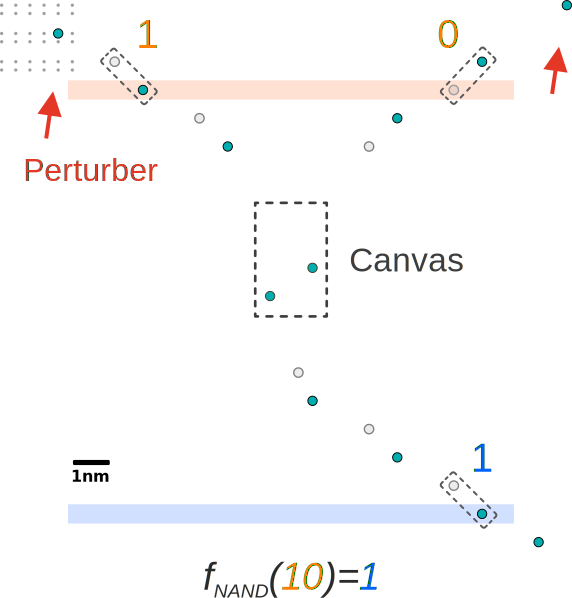
\includegraphics[width=.55\linewidth,valign=c]{figs/nand_10_bestagon_gate.pdf}
        \label{sfig:sidb-logic-hex-tile}
    }
    \caption{
        (\textbf{a}) A logic unit cell made of a pair of \glspl{sidb} sharing a single negative charge~\cite{huff2018binary} simulated in \emph{SiQAD}~\cite{ng2020siqad}. \textbf{Top:} the unit cell is illustrated without charges for readability; \textbf{middle:} unit cell simulated with charge, alongside an additional \gls{sidb} placed to the right (dubbed a \textit{perturber}), biasing the unit cell to take on logic state $0$; \textbf{bottom:} like above but with the perturber moved to the left, biasing the unit cell to take on logic $1$. Reprinted from~\cite{ng2023blueprint} with permission.
        (\textbf{b}) A NAND gate from the \emph{Bestagon} library~\cite{walter2022hexagons} which defines standard locations for I/O pins and a canvas at the center which allows flexible placement of \glspl{sidb} to implement logic gates. Input pins are located at the top with input logic states set by input perturbers---a closer perturber pushes the input wire to the logic $1$ position, while a further one allows charges to take on logic $0$ state. The output is read out at the output pin located at the bottom. Adapted from~\cite{drewniok2025quicktrace} with permission.
    }
    \label{fig:sidb-logic}
\end{figure}

\OLD{\glspl{sidb} can be manufactured on the surface of hydrogen-passivated Silicon(100)-2$\times$1 by removing each hydrogen atom with the tip of a scanning-tunneling microscope, whereby the application of a current near a hydrogen atom desorbs it from the surface, leaving behind a vacancy~\cite{achal2018lithography, pitters2024atomically}; \glspl{sidb} can also be erased by reintroducing a hydrogen atom to the vacancy with a functionalized tip~\cite{huff2017atomic}.
Each \gls{sidb} can hold discrete charge states---negative, neutral, or positive---that is determined by bulk doping level and external electrostatic influences~\cite{pitters2024atomically}.
Charges can be shared among \glspl{sidb} in close proximity, thus allowing closely-spaced \gls{sidb}-pairs to represent binary logic states based on the location of the charge in the \gls{sidb}-pair, as illustrated in \fref{sfig:sidb-logic-pairs}. Ensembles of these \gls{sidb}-pairs with careful placement have been experimentally proven to implement logic gates, such as the $5 \times \SI{6}{\nm^2}$ OR gate which employs two \gls{sidb} pairs as inputs and one \gls{sidb} pair as output~\cite{huff2018binary}.
\gls{cad}-assisted explorations have continued to push the exploration of \gls{sidb} gate and circuit implementations~\cite{ng2020siqad, bahar2020atomic, ahmadpour2023energyaware, vieira2022threeinput}, culminating in the proposal of standard-tile libraries that implement a collection of foundational \gls{sidb} gates with standardized input and output pin locations~\cite{walter2022hexagons}. One such gate from the \emph{Bestagon} gate library is illustrated in \fref{sfig:sidb-logic-hex-tile}~\cite{walter2022hexagons}. The advent of these libraries has enabled the incorporation of \gls{sidb} support in \emph{fiction}~\cite{walter2019fiction, walter2022hexagons}, which provides a suite of tools that enable \gls{eda} for \gls{fcn} technologies including technology mapping, placement and routing, exporting technology-specific designs via gate libraries, and more. \emph{fiction}'s capabilities allow this work to synthesize gate-level Verilog descriptions down to quantum-dot level layout descriptions that are supported by \emph{SiQAD}~\cite{ng2020siqad}, a specialized \gls{cad} tool for \gls{sidb} logic design and simulation.}


%%%%%%%%%%%%%%%%%%%%%%%%%%%%%%%%%%%%%%%%%%%%%%%%%%
% Background
%%%%%%%%%%%%%%%%%%%%%%%%%%%%%%%%%%%%%%%%%%%%%%%%%%
\section{Related Work} \label{sec:related-work}

\begin{figure}
    \centering
    \subfloat[\gls{mxu} systolic array.]{
        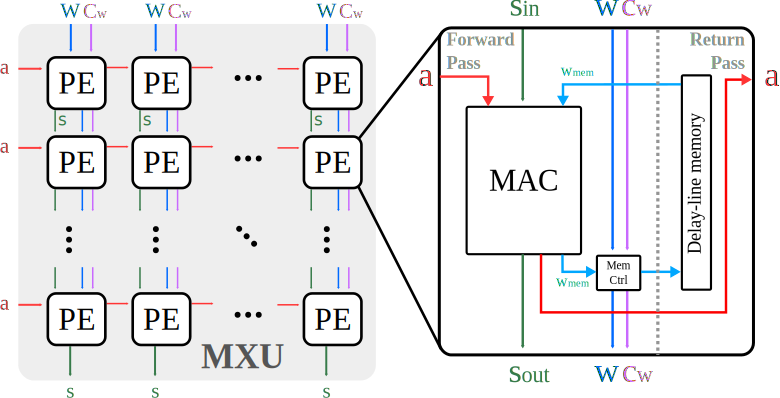
\includegraphics[width=.45\linewidth]{figs/mxu_sa_colored.pdf}
        \label{sfig:schem_mxu_flow_sa}
    }\quad
    \subfloat[PE internal layout.]{
        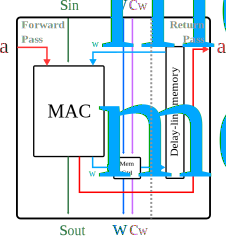
\includegraphics[width=.45\linewidth]{figs/mxu_pe_layout.pdf}
        \label{sfig:schem_pe}
    }
    \caption{
        \bpar{a} A systolic array \gls{mxu} taking in quantized activations ($a$), weights ($w$), weight control signals ($C_w$), and partial sums ($s$). Adapted from~\cite{ng2023blueprint} with permission.
        \bpar{b} Layout within a \gls{pe} showing key components: \gls{mac} arithmetic unit, memory controller, and delay-line memory for weight storage. The signal paths are also illustrated, showing that signals propagate downwards on the left side of the \gls{pe} and upwards on the right side, the two sides are thus dubbed the forward- and return-passes.
    }
    \label{fig:mxu-systolic-array}
\end{figure}

\OLD{Out of the scarce selection of application-scale \gls{sidb} implementations, the proposed blueprint of an \gls{sidb} \gls{mxu}~\cite{ng2023blueprint} intended to accelerate matrix-multiply operations in machine learning applications forms the basis for this work. The implementation took inspiration from key design choices from Google's \gls{tpu}v1~\cite{jouppi2017indatacenter}, including the use of 8-bit quantized integer arithmetic in lieu of floating point operations to reduce compute costs, and a systolic array architecture for efficient data flow which works well with matrix multiplication. Systolic arrays consist of regular arrangements of \glspl{pe}---compute modules that share the same design, arranged in a way to operate on its inputs and pass the results onto the next \gls{pe}. In the blueprint, each \gls{pe} performs the \gls{mac} operation which can be written as~\cite{ng2023blueprint}:}
%
\begin{equation}
    s_{\text{out}} = s_{\text{in}} + (a \times w),
\end{equation}
%
\OLD{where $s_{\text{in}}$ is the input partial sum computed by a prior \gls{pe}, $a$ is the activation, $w$ is the weight, and $s_{\text{out}}$ is the output partial sum. \fref{sfig:schem_mxu_flow_sa} illustrates the systolic array layout of the \gls{sidb} \gls{mxu} and associated high-level data flow.}

\OLD{The \gls{mxu} has two modes of operation:
%
% somehow enabling enumitem throws an error, so we'll do inline enumerates with this workaround
%
\mbox{1) preloading}, where weights ($w$) are loaded into the systolic array from the top until they reach their destined \glspl{pe}, upon which they're stored in the corresponding \gls{pe}'s memory; and
\mbox{2) computing}, where activations ($a$) are loaded into the systolic array from the side for the \gls{mac} operation to be carried out in the \glspl{pe}. Activations continue traversing rightward, multiplying with subsequent weights, while partial sums ($s$) traverse downward to be summed with the next $a \times w$ product.}

\OLD{At a more fine-grained level, each \gls{pe} must be able to determine the operation mode based on input flags, and perform \gls{mac} computation when operating in the computing mode. Key components in each \gls{pe}, including the \gls{mac} unit and the memory controller, can be designed and arranged such that most operations are performed combinationally with unidirectional signal flow; some signals must subsequently flow in the reverse direction to complete the \gls{pe}. \fref{sfig:schem_pe} illustrates this arrangement of components in the \gls{pe}, with all of the logical operations performed on the left side of the \gls{pe} when signals flow from top to bottom, while reverse signals on the right side allow activations to be passed to the neighboring tile and the stored weight in the delay-line memory to be passed back to the \gls{mac}'s input. We dub the left side the \textit{forward-pass} and the right side the \textit{return-pass} in reference to the direction of signal propagation.
The implementation is deeply pipelined, a trait that is common among \gls{fcn} technologies in consideration of operational reliability and in order to facilitate signal propagation. This means that, at each clock cycle, different inputs can be interleaved to increase the computational throughput of the \gls{mxu}.
The blueprint used logic components which were proven in simulation as the basis to approximate the dimensions of larger components~\cite{ng2023blueprint}, which includes various foundational two-input, one-output logic gates and a half-adder introduced in~\cite{ng2020siqad} without the use of standard-tile libraries.}

\OLD{The prior work reported up to $10\times$ improvement in area efficiency and up to $10^8\times$ in power efficiency when compared against Google's \gls{tpu}v1~\cite{ng2023blueprint, jouppi2017indatacenter}. However, the approximated nature of the proposal means that it offers neither an exact \gls{sidb} layout that can be manufactured and tested, nor any verification in operational correctness.}

\OLD{To this end, our work harvests latest \gls{fcn} \gls{eda} techniques to bridge the gap in the verification of logic designs and the lack of accurate physical layouts in \gls{sidb} applications by implementing the \gls{pe} in Verilog, verifying fully pipelined interleaved operations with test benches, and demonstrating a design flow that synthesizes the description to dot-accurate \gls{sidb} layouts, as detailed in the following section.}


%%%%%%%%%%%%%%%%%%%%%%%%%%%%%%%%%%%%%%%%%%%%%%%%%%
% Methodology
%%%%%%%%%%%%%%%%%%%%%%%%%%%%%%%%%%%%%%%%%%%%%%%%%%
\section{Methodology} \label{sec:methodology}

\OLD{In this section, we describe the full methodology at the core of this work. Starting with \secref{sec:methodology-verilog}, we discuss our hierarchical Verilog development approach which satisfies \mbox{1) the} restrictions on input netlists imposed by \gls{fcn} \gls{eda} tools and \mbox{2) our} desire to verify the operational correctness of the \gls{sidb} \gls{mxu}; then in \secref{sec:methodology-eda}, we present the workflow employed by this work to map the \gls{rtl} Verilog all the way down to synthesized quantum-dot layouts.}

\subsection{\titlecap{\glsentrylong{mxu} in Hierarchical Verilog}}\label{sec:methodology-verilog}

\begin{algorithm}[tbp]
\footnotesize
\caption{Processing Element's Forward Pass Logic}\label{alg:pe-forward}

\renewcommand{\algorithmicrequire}{\textbf{Inputs:}}
\renewcommand{\algorithmicensure}{\textbf{Outputs:}}

\begin{algorithmic}[1]
    \newcommand{\codecomment}[1]{\textit{\textcolor{gray}{// #1}}}
    \Require
    \Statex $\mathit{PE}_{y} \gets$ y-index assigned to each PE (constant per PE)
    \Statex $m \gets$ PRELOAD (0) or COMPUTE (1) mode
    \Statex $w_\text{load} \gets$ weight to be loaded into memory
    \Statex $\mathit{PE}_{\text{target-}y} \gets$ target Y-index of $w_\text{load}$
    \Statex $s_\text{in} \gets$ input partial product
    \Statex $a \gets$ input activation
    \Statex $w_\text{mem} \gets$ weight loaded from delay-line memory

    \Ensure
    \Statex $s_\text{out}$: new partial sum
    \Statex $w_\text{mem-out}$: weight to write to delay-line memory

    \Procedure{ProcessingElementLogic}{}
    \State $p \gets \text{signed}(w_\text{mem}) \times \text{signed}(a)$\Comment{Multiply stored $w$ with $a$}
    \State $p_\text{signExtended} \gets \text{signExtend}(p, 24)$
    \State $s_\text{out} \gets s_\text{in} + p_\text{signExtended}$\Comment{Sum with partial sum}
    \If{$m = \text{PRELOAD}$ \textbf{and} $PE_{\text{target-}y} = PE_{y}$}
       \State $w_\text{mem-out} \gets w_\text{load}$\Comment{Update stored weight}
    \EndIf
    \State \Return $s_\text{out}$, $w_\text{mem-out}$, and other pass-through wires
    \EndProcedure
\end{algorithmic}
\end{algorithm}

\OLD{We approach the Verilog implementation of the \gls{mxu} with the following requirements in mind:
%
\begin{enumerate}
    \item The Verilog implementation must obey the constraints of \emph{fiction}, which expects combinational gate-level netlists as inputs, with no feedback loops or registers. Signal flow in the placed and routed \gls{sidb} layouts would also be unidirectional.
    \item Operation of the pipelined processing element must be verifiable---whereas prior work on the \gls{sidb} \gls{mxu}~\cite{ng2023blueprint} did not include formal verifications of the \gls{mxu}'s operation, this work has the opportunity to verify our Verilog implementation with test bench coverage.
\end{enumerate}
%
As described in \secref{sec:related-work}, each \gls{pe} in the \gls{sidb} \gls{mxu} includes a forward pass where most of the core logic takes place, and a return pass which is required for signal synchronization and the operation of the delay-line memory. However, this creates a feedback loop which violates \emph{fiction}'s input expectations. To work around this, our \gls{rtl} Verilog implementation is split hierarchically. The core logic in the forward pass is implemented as a combinational Verilog description and shown in Alg.~\ref{alg:pe-forward}. Operation of the full \gls{pe} is then captured by a higher level \gls{rtl} Verilog description that defines the component's input and output signals, pipelined internal signal steering, and synchronized signal timing for the return pass.}

\OLD{Test benches can thus be written for both levels of Verilog descriptions. At the lower level, test benches have been implemented to verify correct \gls{mac} operation with signed numbers, including edge cases like inputting large signed integers that verify proper operation at the limit of the 8-bit quantized implementation. At the full \gls{pe} level, test benches have been written to verify operation in preloading and compute modes. Since it is expected that the final \gls{sidb} implementation would be deeply pipelined, the test benches also verify pipelined operation by presenting interleaved inputs across multiple clock cycles to verify the \gls{pe}'s ability to handle multiple sets of weights and activations simultaneously going through different pipeline stages.
Simulations are performed using Icarus Verilog~\cite{icarusverilog}. These test benches ensure that the PE design is logically correct before proceeding to synthesis and physical mapping.
You can find the full open-source Verilog implementation on GitHub~\cite{githubsupplementary}.}


\subsection{Design Automation Workflow}\label{sec:methodology-eda}

\OLD{
After verifying the Verilog description, the \gls{rtl} design must be synthesized into a gate-level netlist in order for \emph{fiction} to process the design. We use Yosys~\cite{wolf2013yosys} to synthesize the \gls{rtl} Verilog description into an \gls{aig} netlist and ABC's \textit{\&deepsyn}~\cite{brayton2010abc} optimization strategy to reduce the network's node count. The resulting gate-level Verilog is then provided to \emph{fiction}~\cite{walter2019fiction} for synthesis to an \gls{sidb} layout using its \gls{fcn}-specific \gls{eda} tooling in the following multi-step process:
%
\begin{enumerate}
    \item Technology mapping is conducted to map the \gls{aig} into gates that are available in the \emph{Bestagon} gate library~\cite{walter2022hexagons}, which further reduces the node count via the expressive power of a full gate library over AND/INV primitives.
    \item Placement and routing with the \textit{ortho} algorithm~\cite{walter2019scalable} produces a layout on a Cartesian grid representing the full logic implementation with valid gate placements that are connected by wires.
    \item Post-layout optimizations are run to reduce the footprint of the layout~\cite{hofmann2023postlayout, hofmann2024late}.
    \item The Cartesian layout is then remapped onto a hexagonal grid~\cite{hofmann2023scalable} in preparation for applying the \emph{Bestagon} library.
    \item SAT-based equivalence checking~\cite{walter2020verification} is performed to verify that the mapped, optimized, and hexagonalized layout faithfully implements the gate-level Verilog specification.
    \item The \emph{Bestagon} library~\cite{walter2022hexagons} is applied to the hexagonalized layout, yielding a dot-accurate \gls{sidb} implementation of the design.
\end{enumerate}
}

\OLD{As part of this investigation, we have also contributed various improvements to \emph{fiction} to further optimize the \gls{eda} tools for \gls{sidb} workflows.
Recent works on \gls{sidb} logic robustness have culminated into the proposal of unified \glspl{fom} for \gls{sidb} gates~\cite{drewniok2024unifying}, which comprehensively capture currently known cost functions that can impact the robustness of \gls{sidb} gates: operational domain size~\cite{ng2020siqad, walter2023reducing}, thermal resilience~\cite{drewniok2023temperature}, band bending~\cite{pitters2011charge}, defect~\cite{ng2024simulating, huff2019electrostatic, croshaw2020atomic}, and more. The scores achieved by each metric are weighted and averaged to obtain $\chi$, a \gls{fom} assigned to the gate. Our gate library uses $\chi$ as the cost function for the technology mapper that will thus favor the most stable gates even if a certain logic could have been implemented with fewer, albeit less stable, selection of gates.
The impact of this in the final layout will be compared in \secref{sec:results-and-discussion}.}

\OLD{We have also improved the hexagonalization step to better align with \gls{sidb} layout expectations. The Cartesian layout prior to hexagonalization employs the 2DDWave clocking scheme~\cite{vankamamidi2008twodimensional} where all input pins are placed along the top and left borders, and signals subsequently flow diagonally from top-left to bottom-right. In prior implementations of hexagonalization, the Cartesian layout is then rotated by $45^\circ$ and projected onto a hexagon grid~\cite{hofmann2023scalable} such that signals flow top-down. As a result, input pins on the hexagonal layout tend to have a $y$ offset from the top. This can negatively impact the theoretical throughput of the layout as some input pins might have to be held at the same value over multiple clock cycles in order to synchronize with other inputs.
These constraints can be alleviated by extending all input pins to the top edge of the layout; we have thus updated the hexagonalization algorithm to perform this extra step which yields fully synchronized circuit layouts.}


%%%%%%%%%%%%%%%%%%%%%%%%%%%%%%%%%%%%%%%%%%%%%%%%%%
% Results and Discussion
%%%%%%%%%%%%%%%%%%%%%%%%%%%%%%%%%%%%%%%%%%%%%%%%%%
\section{Results and Discussion}\label{sec:results-and-discussion}

\begin{table*}
    \centering
    \caption{\OLD{Placed and Routed MXU Processing Element (Forward Pass)}}
    \label{tab:pe-results}
    \begin{tabular}{lccccccc}
    \toprule
    Experiment & Tiles ($w \times h$) & Physical dimensions (\si{\nm^2}) & Gates & Wires & Crossings & \glspl{sidb} \\
    \midrule
    All gates equally preferred & $515 \times 1043$ & $\num{30930} \times \num{35474}$ & \num{613}  & \num{120945} & \num{11880} & \num{1645777} \\
    \gls{fom}-informed & $516 \times 1049$ & $\num{30990} \times \num{35678}$ & \num{607}  & \num{124048} & \num{11057} & \num{1685608} \\
    \bottomrule
    \end{tabular}
\end{table*}

\begin{table*}[!t]
  \caption{Comparative experimental evaluation of the synthesized \gls{sidb} layouts across different synthesis approaches. \TODO{Rephrase title, fill table with actual details}}
  \centering
  \label{tab:benchmarks_ortho}
  \begin{minipage}{\linewidth}
    \centering
    % \resizebox{\linewidth}{!}{
      \begin{tabular}{l@{\hskip 6pt}l@{\hskip 6pt}r@{\hskip 2pt}c@{\hskip 2pt}l@{\hskip 6pt}c@{\hskip 6pt}rcrr}
        \toprule
        \multirow[c]{2}{*}{\makecell[tl]{\textsc{Experiment}}} &
        \multirow[c]{2}{*}{\makecell[tl]{\textsc{Algorithm}}} &
        \multicolumn{5}{c}{\textsc{Tiles}} &
        \multicolumn{1}{c}{\textsc{Dimensions}} &
        \multirow[c]{2}{*}{\makecell[tl]{$|\text{SiDBs}|$}} &
        \multirow[c]{2}{*}{\makecell[tl]{\textsc{$t\,[s]$}}} \\
        \cmidrule(lr){3-7} \cmidrule(lr){8-8}
         & &
        $w$ & $\times$ & $h$ & $=$ & $A$ & \multicolumn{1}{c}{\textsc{W $\times$ H [\si{\nm} $\times$ \si{\nm}]}} &  & \\
        \midrule
        % --- Hand-designed baseline
        {Blueprint~\cite{ng2023blueprint}} & Hand made &
        -- & $\times$ & -- & $=$ & -- & \num{5000} $\times$ \num{8150} & -- & -- \\
        % --- IEEE-NANO baseline
        {Unspecified \glspl{alu}~\cite{ng2025building}} & \emph{ortho} + \emph{PLO} &
        \num{515} & $\times$ & \num{1043} & $=$ & \num{537145} & $\num{11877} \times \num{13622}$ & \num{1645777} & \num{91} \\
        % --- New
        \multirow[t]{2}{*}{\makecell[tl]{Optimized \glspl{alu}\\(This work)}} & \TODO{} &
        -- & $\times$ & -- & $=$ & -- & -- $\times$ -- & -- & -- \\
        & \TODO{} &
        -- & $\times$ & -- & $=$ & -- & -- $\times$ -- & -- & -- \\
        % --- DATE for our own reference, delete before submission
        % \multirow[t]{4}{*}{\makecell[tl]{BitNet b1.58 MXU\\(This work)}} & \emph{ortho} &
        % \num{154} & $\times$ & \num{372} & $=$ & \num{57288} & $\num{3559} \times \num{4861}$ & \num{263431} & $<\!1$\\
        % & \emph{ortho} + \emph{PLO} &
        % \num{98} & $\times$ & \num{233} & $=$ & \num{22834} & $\num{2269} \times \num{3046}$ & \num{178778} & \num{1078}\\
        % & \emph{gold} &
        % \num{87} & $\times$ & \num{190} & $=$ & \num{16530} & $\num{2016} \times \num{2485}$ & \num{133882} & \num{37}\\
        % & \emph{gold} + \emph{PLO} &
        % \num{86} & $\times$ & \num{184} & $=$ & \num{15824} & $\num{1993} \times \num{2407}$ & \num{132041} &\num{51}\\
        \bottomrule
      \end{tabular}
    % }
    \begin{minipage}{\linewidth}
      \vspace{0.5em}
      Runtime values are in seconds; $w$, $h$, and $A$ are the width, height, and resulting area (in tiles) of the layout, respectively; dimensions refer to the area footprint of the synthesized \gls{sidb} layout after applying the Bestagon gate library \cite{walter2022hexagons}; $|\text{SiDBs}|$ indicates the number of \glspl{sidb}. \TODO{Add columns: FoM Awareness, HA Used (if applicable)} \TODO{Add footnote to Blueprint area that it's for the full PE, whereas the rest are only for the PE-forward path.}
    \end{minipage}
  \end{minipage}
\end{table*}

\OLD{Following the \gls{eda} workflow laid out in \secref{sec:methodology-eda}, we have successfully synthesized the \gls{rtl} Verilog description of the forward-pass \gls{pe} all the way down to a dot-accurate \gls{sidb} layout. We present the results in \tref{tab:pe-results}, which includes: the network dimension in terms of tile count, the physical dimension in \si{\nm^2}, as well as the counts of gates, wires, crossings, and \glspl{sidb} used in the layout. Note that in this table, every tile that is mapped to a wire in the final layout is counted as 1 wire, thus a single wire signal that spans across $10$ tiles would increment the value by $10$.
We can see that the layout resulting from \gls{fom}-informed technology mapping is slightly larger than the simpler alternative of treating all gates with equal preference, indicating that the technology mapper has indeed chosen costlier solutions that make use of more robust gates. This area trade-off comes with the benefit that \gls{sidb} gates with higher reliability metrics are more often employed in the layout, which can ultimately yield a more robust device. It is also important to note that the \gls{fom} values from~\cite{drewniok2024unifying} are derived from a specific variant of the \emph{Bestagon} library optimized under a particular set of physical conditions. Choosing different libraries or physical conditions may yield different trade-offs.
Also notable is that the original hexagonalization algorithm would have imposed a $\frac{1}{12}\times$ throughput limit compared to full throughput, a limitation that is now alleviated by extending the input pin wires (as discussed in \secref{sec:methodology-eda}) at no increase in area cost.}

\OLD{Although the synthesized \gls{sidb} layout only covers the forward pass of the \gls{pe}'s operation, it already represents all of the logic operations; the parts that are not included in the synthesized layout are purely for signal propagation, as described in \secref{sec:methodology-verilog}. We thus believe that there is value in comparing our results with the previously proposed blueprint~\cite{ng2023blueprint}. The blueprint reported an area footprint of $5000 \times \SI{8150}{\nm^2}$, which means that the area we've achieved is $\sim30\times$ higher than those estimated by the blueprint, and the gap would further widen if we were to synthesize the entire \gls{pe}. Why is there such a substantial increase in area compared to previous estimates?}

\OLD{We believe there are multiple contributing factors. Whereas the previously proposed blueprint used hand-designed components with fairly high logic gate density~\cite{ng2023blueprint, ng2020siqad}, this work uses the \emph{Bestagon} gate library which deliberately chose a large tile template to ensure sufficient separation between the logic canvas of neighboring logic tiles in order to minimize inter-gate interference~\cite{walter2022hexagons}. Furthermore, the blueprint study benefited from deliberately chosen multiplier and adder implementations that were, themselves, systolic array designs optimized for \gls{fcn} implementation. In this study, the choice of arithmetic unit implementation is completely left to Yosys and ABC's synthesis tools, which are optimized for traditional CMOS devices with very different architectural trade-offs. Furthermore, once we perform logic optimization with ABC, the boundaries of arithmetic elements get completely blurred, hindering the possibility of potential optimization algorithms that could benefit from such arithmetic knowledge.
Lastly, due to the large size of the netlist required by this application (in relation to other \gls{fcn} applications), it is computationally intractable to use the optimal placement and routing algorithms offered by \emph{fiction} such as the \textit{exact}~\cite{walter2018exact} and \textit{gold}~\cite{hofmann2024born} solvers. Instead, we had to rely on algorithms which prioritized runtime at the sacrifice of final area cost.
Nevertheless, the successful end-to-end design flow achieved by this study presents an encouraging demonstration of what state-of-the-art \gls{fcn} \gls{eda} tools can achieve on the \gls{sidb} platform, highlighting opportunities for further optimization.}


%%%%%%%%%%%%%%%%%%%%%%%%%%%%%%%%%%%%%%%%%%%%%%%%%%
% Future Work
%%%%%%%%%%%%%%%%%%%%%%%%%%%%%%%%%%%%%%%%%%%%%%%%%%
\section{Conclusion and Future Work}\label{sec:conclusion-future-work}

\OLD{In past studies, the design and verification of large-scale SiDB applications remained disconnected from their physical implementations, constrained by immature \gls{eda} tooling and manually-intensive workflows at the time~\cite{chiu2020thes, ng2023blueprint}. Enabled by recent advances in \gls{sidb}-focused \gls{eda} frameworks, this work presents the first automated, end-to-end design flow for implementing a processing element (\gls{pe}) of a \gls{sidb}-based \glsentrylong{mxu} designed specifically for machine learning acceleration.
Our hierarchical Verilog structure facilitates the synthesis of combinational components down to the \gls{sidb} level while enabling validation of the complete operational functionality through higher-level \gls{rtl} modules. By strategically separating core combinational logic from higher-level pipeline control, we successfully synthesized a majority of the \gls{pe}'s functionality into a dot-accurate \gls{sidb} layout, selectively omitting specific signal components from synthesis to accommodate \gls{eda} tooling restrictions. Although the synthesized layout exhibits a larger area compared to previous hand-crafted designs~\cite{ng2023blueprint}, our effort provides a concrete demonstration of automated design methodologies applied to \gls{sidb}-based circuits, and underscores opportunities for further optimizations in \gls{sidb}-specific \gls{eda} flows. Additionally, this study is the first to incorporate \gls{fom} considerations into \emph{fiction}'s technology mapping process, prioritizing gate reliability within synthesized layouts.}

\OLD{One limitation faced by this study is the lack of control over the implementation of fundamental arithmetic units such as adders and multipliers. Since the design trade-offs of \gls{sidb} logic differ significantly from CMOS designs, it is possible that our workflow for synthesizing \gls{rtl} Verilog to gate-level Verilog using established tools like Yosys and ABC is introducing unnecessary overhead due suboptimal implementation choices. Further improvements to this synthesis step, as well as further developments to \emph{fiction}'s placement and routing algorithms, can bridge the gap between synthesized layouts and expert-designs and incentivize further development of novel applications optimized for \glspl{sidb}.}


%%%%%%%%%%%%%%%%%%%%%%%%%%%%%%%%%%%%%%%%%%%%%%%%%%
% Bibliography
%%%%%%%%%%%%%%%%%%%%%%%%%%%%%%%%%%%%%%%%%%%%%%%%%%
\bibliographystyle{IEEEtran}
\bibliography{zotero_refs_2025_et_al,manual_refs}
% zotero_refs.bib: original bib file exported from Zotero
% zotero_refs_normalized.bib: modified bib file where author fields with >6 authors are converted to et al



\end{document}
